\chapter{El transistor}\label{chapter:transistor}

Antes de la invención del primer transistor a finales de la década de 1930, ya existían dispositivos que cumplían la misma función que 
este pero con una menor eficiencia.\\
\indent A finales del siglo XIX con el incipiente desarrollo de la tecnología de comunicación inalámbrica y la construcción de sistemas que
utilizaran este método por la \emph{compañía Marconi}, \emph{Guglielmo Marconi} le asignó el cargo de consejero científico al físico
inglés \emph{John Ambrose Fleming}. \emph{Marconi} necesitaba ayuda para mejorar el \textbf{detector}, que es el
dispositivo que se encarga de extraer información de una corriente de radiofrecuencia modulada, y aunque ya él había desarrollado un
\textbf{detector magnético}, este solo brindaba una señal de frecuencia de audio a un receptor de teléfono. Un \textbf{detector}
confiable que pudiera guiar un instrumento de impresión era necesario. Fleming pudo desarrollar un \textbf{tubo al vacío} como resultado de su 
trabajo con \textbf{bombillas de efecto Edison}, a estas las denominó \textbf{válvulas de oscilación} ya que pasaba corriente en una sola
dirección. Fleming presentó una patente para estos tubos, cedida a la \emph{compañía Marconi} en el Reino Unido en noviembre de 1904 y esta
se emitió en septiembre de 1905. Conocida más tarde como la \textbf{válvula Fleming}, la \textbf{válvula de oscilación} se desarrolló con el
fin de rectificar la corriente de radiofrecuencia como componente detector de circuitos receptores de radio. \brackcite{wikipedia_2022_tube}\\
\indent En el propio siglo XIX ingenieros de telégrafos y teléfono habían reconocido la necesidad de incrementar la distancia que la señal pudiera ser
transmitida. En 1906 \emph{Robert Von Lieben} solicitó una patente para un \textbf{tubo de rayos catódicos} que usaba una bobina de deflexión
magnética externa y estaba destinado a usarse como amplificador en equipos de telefonía. A \emph{Lee de Forest} se le acredita la invención del
tubo triodo en 1907, el cual tenía la capacidad de amplificar las señales, y que fue el primero de su tipo que tuvo uso práctico. Sin embargo estos
\textbf{tubos de vacío} utilizados para amplificar la música y la voz que hicieron posibles las llamadas de larga distancia, creaban mucho calor y
se quemaban muy rápido, requiriendo alto mantenimiento. \brackcite{wikipedia_2022_tube, wikipedia_2022_triode}\\
\indent La \textbf{ENIAC}(\emph{Electronic Numerical Integrator and Computer}) fue la primera computadora en usar los \textbf{tubos de vacío}, exactamente
18 000 de estos para poder funcionar, que hicieron que aquel dispositivo ocupara el tamaño de una habitación completa. Estos tubos permitían que las
señales fueran enviadas y los cálculos realizados de forma más rápida a través del uso de conmutación eléctrica en vez de conmutación mecánica. 
Debido al enorme consumo de energía eléctrica de la \textbf{ENIAC}, muchas personas creyeron que esta se destruiría, sin embargo los \textbf
{tubos de vacío} le permitieron soportar y funcionar. ~\brackcite{richards_2022}.\\

\begin{figure}[htb]
	\centering
	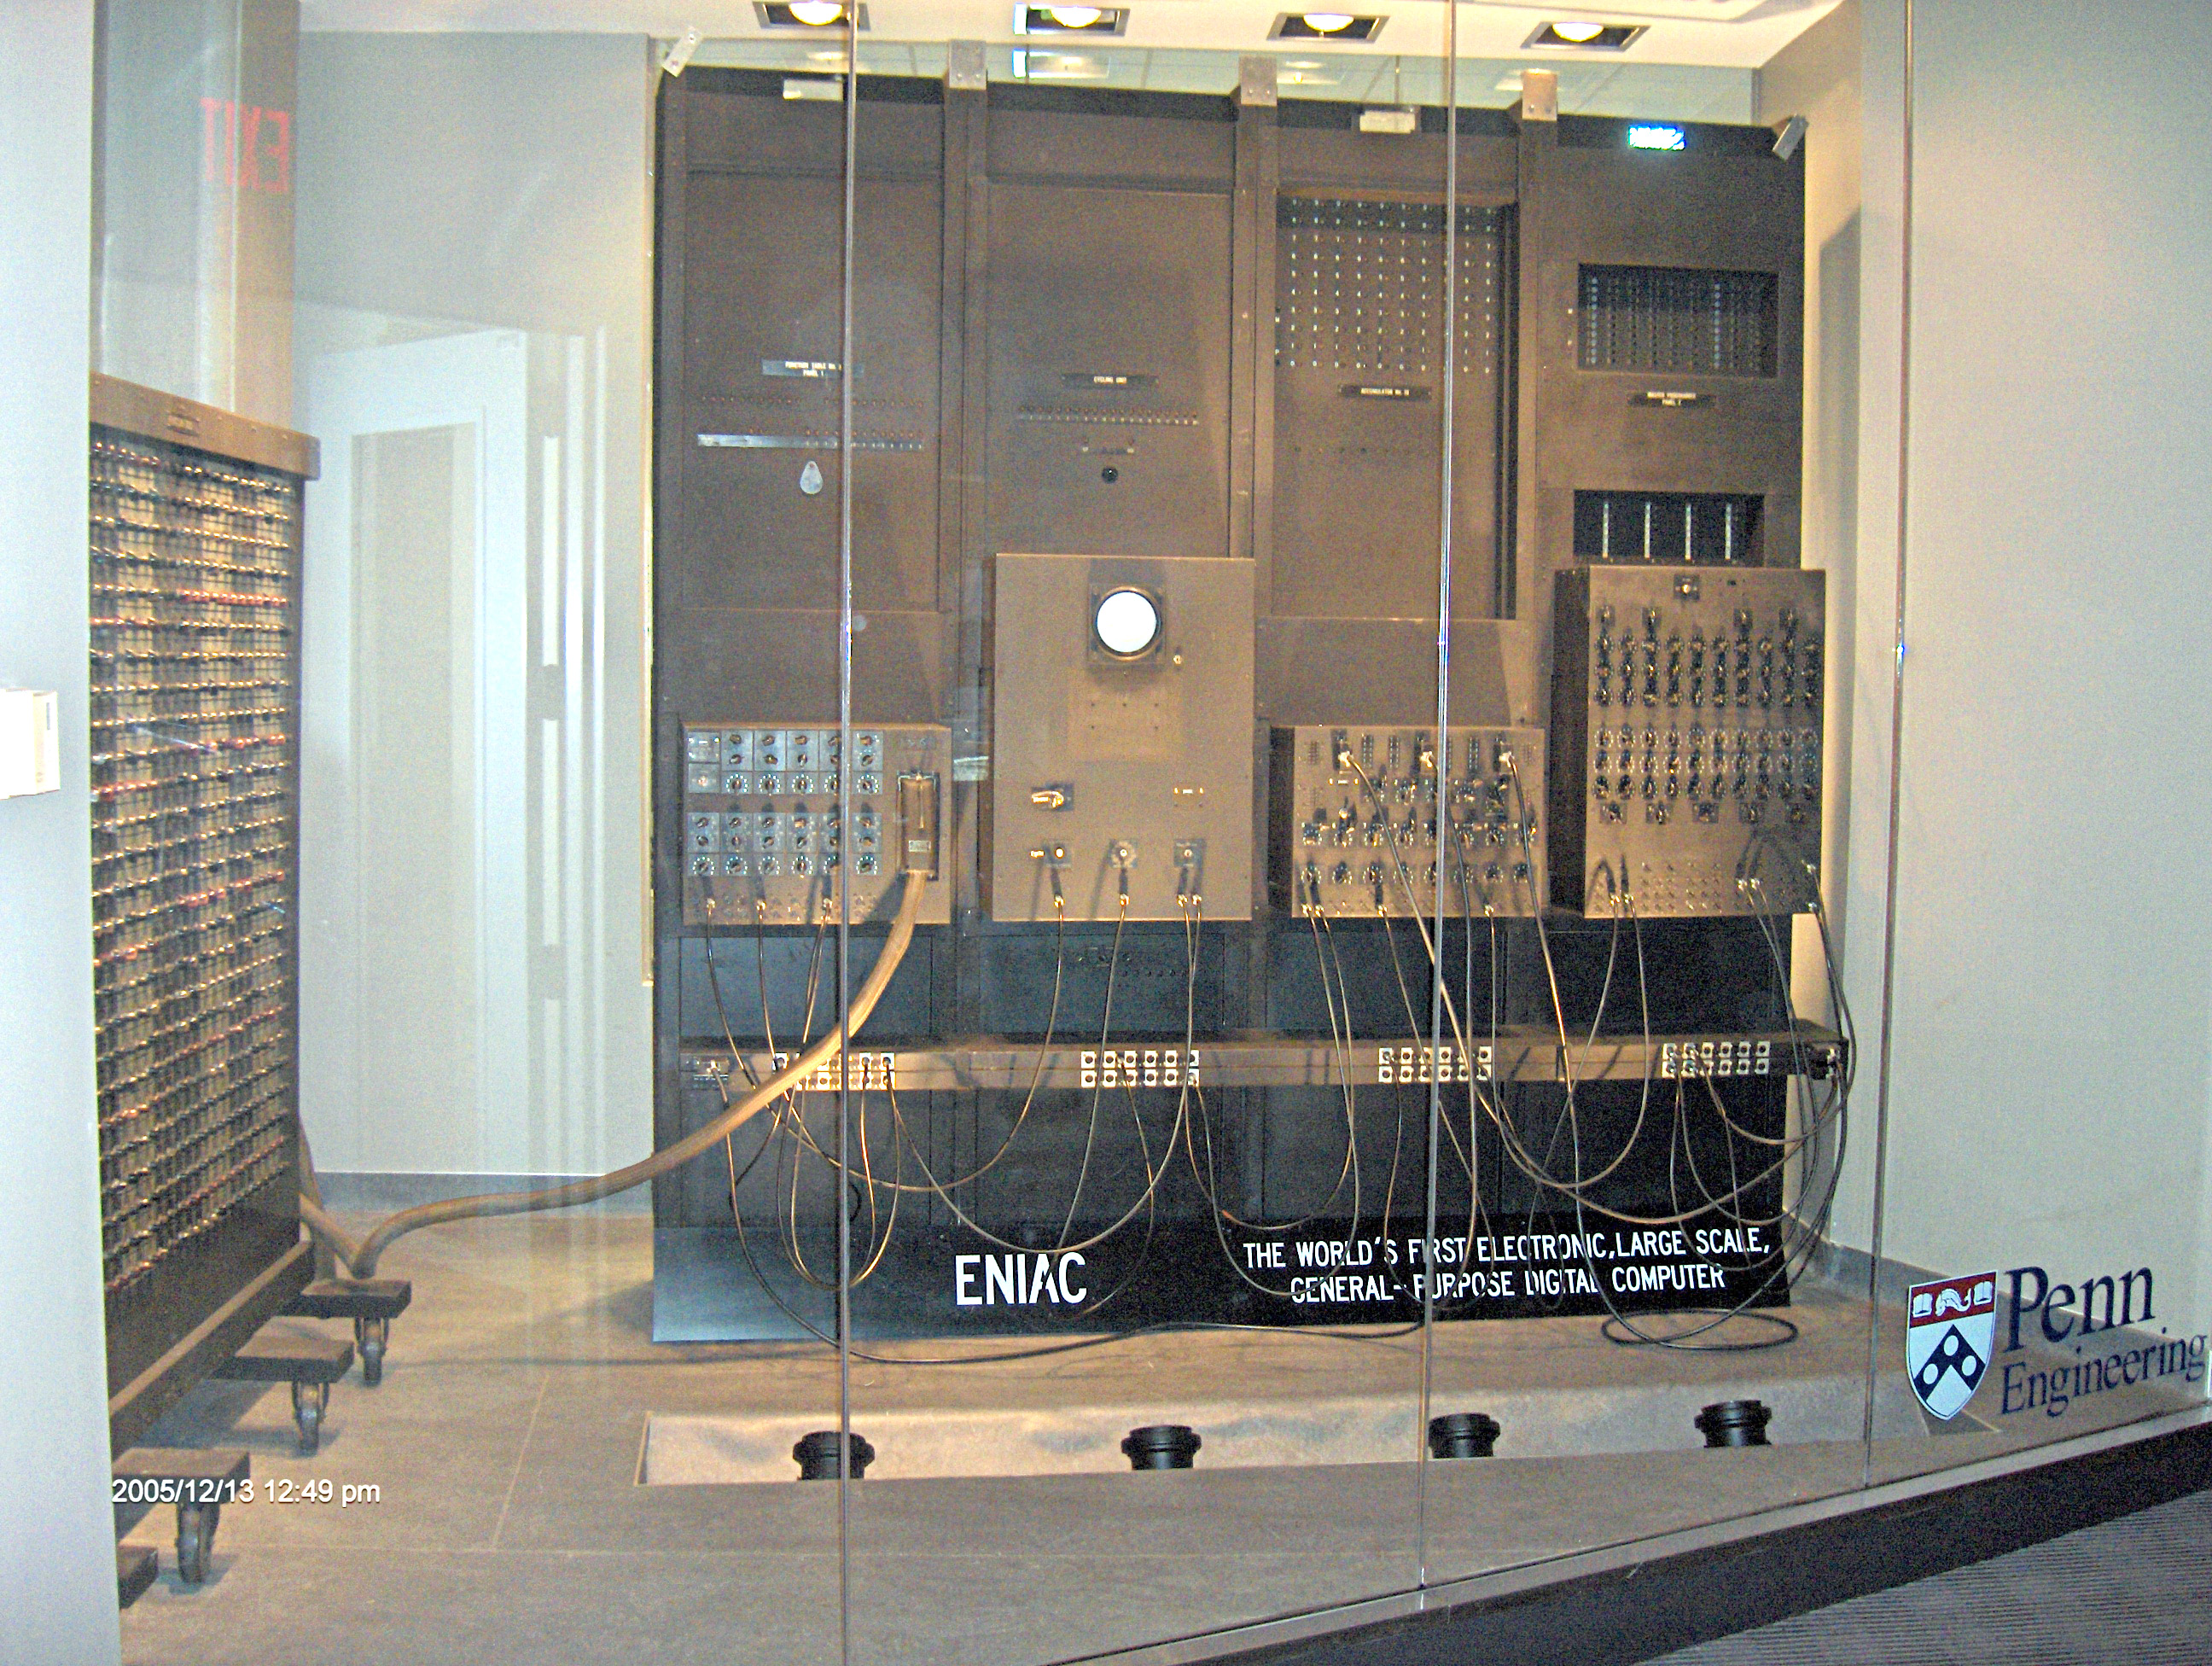
\includegraphics[scale = 0.13]{Graphics/ENIAC.jpg}
	\caption{\textbf{ENIAC} primera computadora que utilizó los \textbf{tubos de vacío}.}
	\label{fig:1}
\end{figure}

\section*{El surgimiento}
Debido a que las computadoras dependían de los \textbf{tubos de vacío} tan frágiles, grandes, costosos y con un consumo enorme de energía, solo las grandes 
compañías, los militares y las universidades con proyectos de investigación podían permitírselas. Por esta razón el inicio de la era digital, aquella donde 
los dispositivos electrónicos se convertirían en una parte indispensable en nuestro día a día, no ocurriría sino hasta el martes 16 de diciembre de 1947. Ese 
día 2 científicos en los \emph{laboratorios Bell} lograron armar un pequeño artilugio que habían inventado a partir de unas tiras de oro, papel de aluminio,
un trozo de material semiconductor y un sujetapapeles doblado, el cual movido a la perfección podía amplificar una corriente eléctrica y encenderla y apagarla.\\
Durante mucho tiempo hubo una persona encargada de encontrar un reemplazo para los \textbf{tubos de vacío}, un reemplazo menos costoso, más sólido y más barato, esa 
persona fue el físico experto en estado sólido \emph{William Shockley}, graduado del \textbf{MIT}(\emph{Massachussets Institute of Technology}), quien fue contratado 
por \emph{Mervin Kelly} jefe del departamente de \textbf{tubos al vacío} de los \emph{labotorios Bell} con este fin. Luego de 3 años a \emph{Shockley} se le ocurrió que 
podría encontrar una solución utilizando materiales sólidos como el silicio en vez de los filamentos de una bombilla, “Se me ha ocurrido que es posible crear un amplificador 
utilizando semiconductores en vez del vacío", escribió \emph{Shockley}. Él tenía la capacidad de visualizar la teoría cuántica, cómo explicaba el movimiento de los
electrones. Sus colegas dijeron que podía mirar material semiconductor y ver los electrones. Sin embargo, para transformar su intuición en un invento real, \emph{Shockley}
necesitaba un socio que fuera un hábil experimentador, y fue \emph{Walter Brattain} quien disfrutaba creando dispositivos con semiconductores quien se unió a \emph{Shockley} en su tarea. 
Lamentablemente sus ideas tuvieron que esperar pues recién comenzó la II Guerra Mundial, y no fue hasta casi 4 años después que regresaron a su trabajo en los laboratorios 
que retomaron su investigación, y fueron asignados a un grupo cuyo objetivo principal era encontrar el tan buscado reemplazo sólido para los \textbf{tubos de vacío} utilizando 
semiconductores.
Los \emph{laboratorios Bell} fueron el fruto de un inmenso trabajo y hasta cierto punto una apuesta de la \textbf{AT\&T}(\emph{American Telephone and Telegraph 
Company}) que a principios de 1907 pasaba por una grave crisis, y con la guía \emph{Alexander Graham Bell}, \emph{Theodore Vail} y el apoyo de la junta directiva
se plantearon el objetivo de conectar las ciudades de \emph{Nueva York} y \emph{San Francisco}, tarea que fue cumplida en enero de 1915 utilizando \textbf{tubos 
de vacío} y nuevas tecnologías para crear amplificadores y repetidores que permitieran cumplir la meta final. Así con el arduo trabajo de muchos expertos y científicos,
y momentos de pura ciencia se crearon las bases de lo que serían luego los \emph{laboratorios Bell}, se había juntado tanto talento en este lugar, teóricos, científicos de
materiales, metalúrgicos, ingenieros e incluso escaladores de postes de \textbf{AT\&T}. Fueron 3 de estos talentosos expertos los que hicieron el descubrimiento el 16 de
diciembre de 1947, el experimentalista sordo \emph{Walter Brattain}, el experto en teoría cuántica \emph{John Bardeen} y , sin embargo la invención del \textbf{transistor} no fue el resultado del trabajo de solo ellos 3, fue la mezcla del conocimiento de diversos talentos presentes 
desde el inicio en los \emph{laboratorios Bell}, e incluso antes. Como escribiera \emph{William Shockley} “Son necesarios muchos hombres de varios campos de la ciencia, 
juntando su talento, para poder llevar a cabo toda la investigación necesaria para el desarrollo de un nuevo dispositivo".\\

\section*{}
